%\documentclass{beamer}
%\usetheme{Pittsburgh} 
\documentclass{scrartcl}

\usepackage[utf8]{inputenc}
\usepackage{default}
\usepackage[procnames]{listings}
\usepackage{graphicx}
%\usepackage[toc,page]{appendix}
\usepackage{caption}
\usepackage{hyperref}
\usepackage{color}
\usepackage{csvsimple}


%Bibliogrpahy?
%\usepackage{bibentry}
%\nobibliography*
%\bibentry{ }


%Java
\definecolor{javared}{rgb}{0.6,0,0} % for strings
\definecolor{javagreen}{rgb}{0.25,0.5,0.35} % comments
\definecolor{javapurple}{rgb}{0.5,0,0.35} % keywords
\definecolor{javadocblue}{rgb}{0.25,0.35,0.75} % javadoc
\lstset{language=Java,
    basicstyle=\ttfamily,
    keywordstyle=\color{javapurple}\bfseries,
    stringstyle=\color{javared},
    commentstyle=\color{javagreen},
    morecomment=[s][\color{javadocblue}]{/**}{*/},
    breaklines = true,
    columns=fullflexible,
    %Numbering and tabs
    %numbers=left,
    %numberstyle=\tiny\color{gray},
    %stepnumber=2,
    %numbersep=1em,
    tabsize=4,
    showspaces=false,
    showstringspaces=false}

\begin{document}

\title{Manual motion observation}
\subtitle{Assignment No. 1}
\author{
  Matin, Maryam \\
  Quignon, Christophe
  %Familyname, Name
} 
\date{\today}


\maketitle



\section{Experimental setup}
\subsection{Robot Design}
%especially how you mark the stop position and how you ensure identical start positions.
\begin{itemize}
\item \href{http://www.damienkee.com/home/2011/8/20/domabot-classroom-robot-design.html}{Domabot}
\end{itemize}

\begin{figure}
 \center
 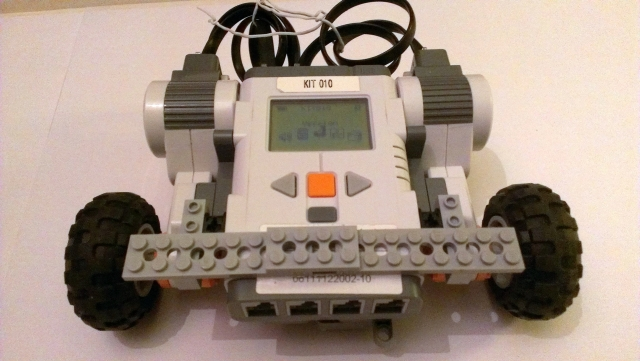
\includegraphics[width= 6cm]{img/robot_front.jpg}
 \caption{The Domabot in front view without pen.}
 \label{fig:front_view}
\end{figure}

\subsection{Execution}
\begin{figure}
 \center
 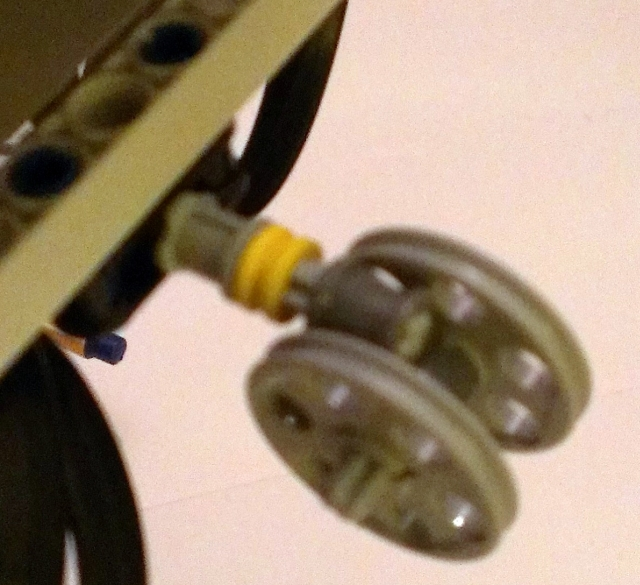
\includegraphics[width= 6cm]{img/steering_wheel.jpg}
 \caption{Detail view of the free wheel}
 \label{fig:free_wheel}
\end{figure}

\begin{itemize}
\item
\end{itemize}

\begin{figure}
\centering
\begin{minipage}{.5\textwidth}
  \centering
  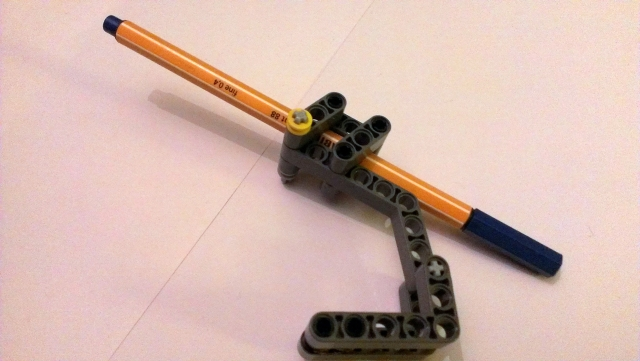
\includegraphics[width=.5\linewidth]{img/pen.jpg}
  \captionof{figure}{Detail view of the pen holder}
  \label{fig:pen}
\end{minipage}%
\begin{minipage}{.5\textwidth}
  \centering
  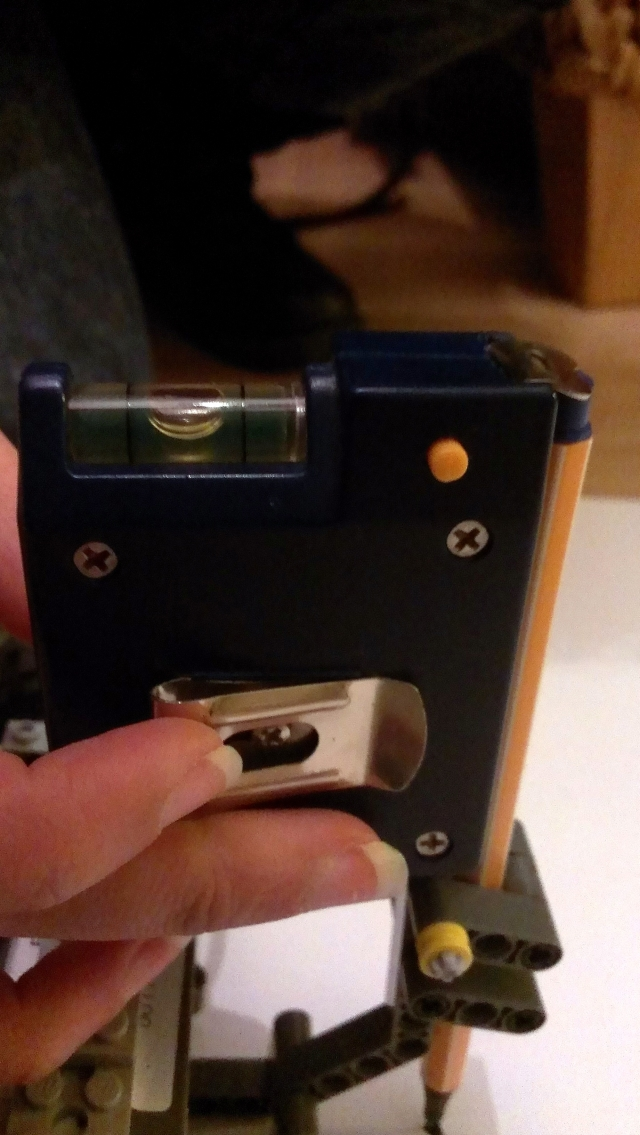
\includegraphics[width=.5\linewidth]{img/pen_adjust.jpg}
  \captionof{figure}{Calibration of the pen/}
  \label{fig:pen_calib}
\end{minipage}
\end{figure}

\begin{figure}
\centering
\begin{minipage}{.5\textwidth}
  \centering
  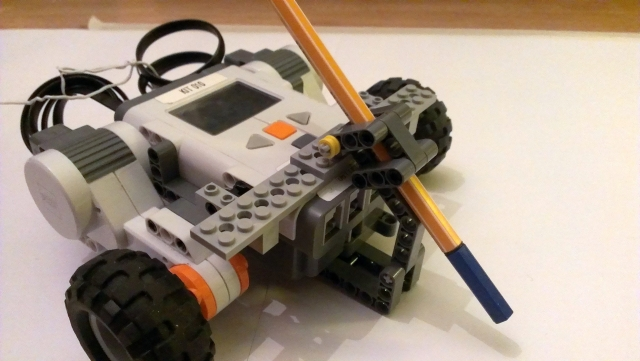
\includegraphics[width=.5\linewidth]{img/pen_up.jpg}
  \captionof{figure}{The Domabot with lifted pen.}
  \label{fig:pen_up}
\end{minipage}%
\begin{minipage}{.5\textwidth}
  \centering
  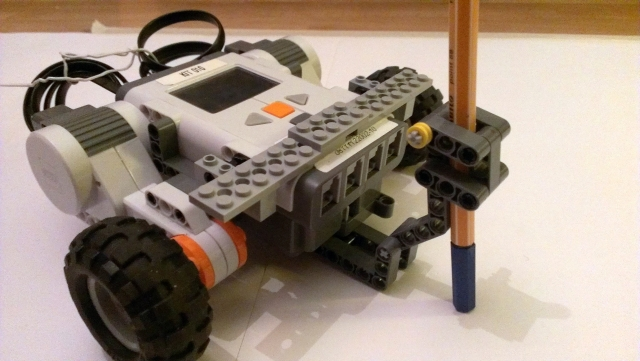
\includegraphics[width=.5\linewidth]{img/pen_down.jpg}
  \captionof{figure}{The Domabot with lowered pen.}
  \label{fig:pen_down}
\end{minipage}
\end{figure}

\section{Observations}
\subsection{Execution}
\begin{figure}
 \center
 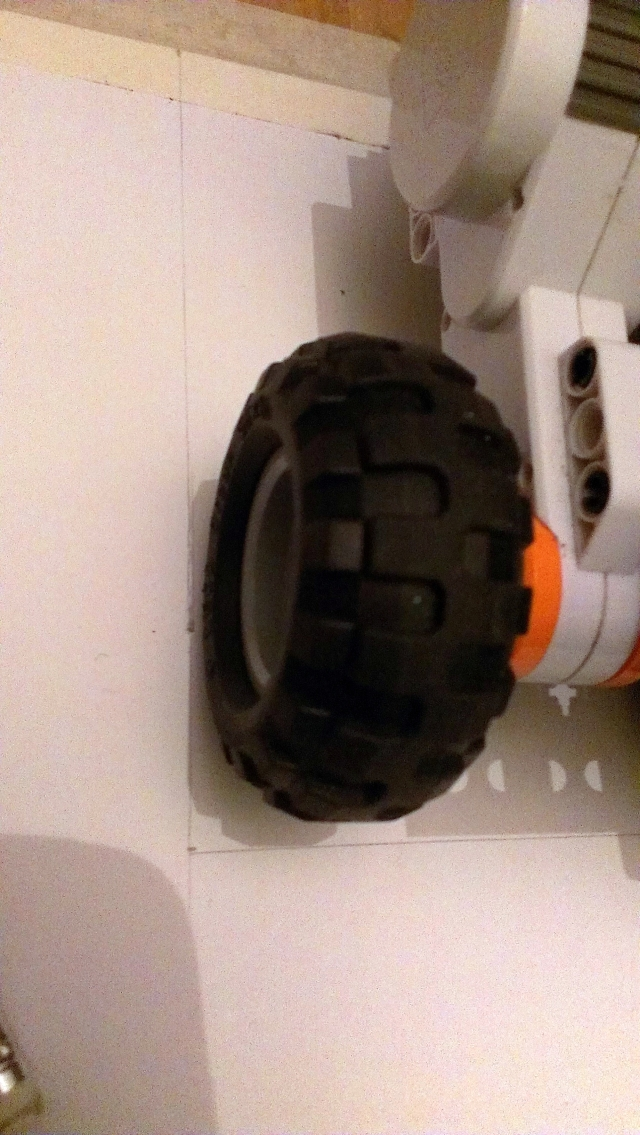
\includegraphics[width= 6cm]{img/wheel_adjust.jpg}
 \caption{The starting position of the Domabot with the help of its shadow.}
 \label{fig:setup}
\end{figure}

\begin{itemize}
\item
\end{itemize}

\section{Observations}



\subsection{Program Parameters}
\begin{itemize}
\item wheelDiameter = 5.6f\\
A wheel diameter is specified as 5.6cm in the Handbook and on the wheel itself.

\item trackWidth = 17.6f\
The track width of the robot, measured in cm.

\item distance = 90.0\\
The distance the robot aims to dive in cm.

\item radius\\
 = $250 * \pi \ 180 * 90 = 392.699$\\
 We decided to go with an angular description of the arc in degree for better understanding and a more meaningful tuning. The function needs a radius in cm as input, but we kept the calculation in the code and thus documented best.

\item Delay.msDelay(500)\\
The direction of turn is selected by pushing a button. Before starting the movement, we wait for half a second, so the operator can remove the finger and the robot can recover from the push.
\end{itemize}


\subsection{Code (see code.java)}
As given in code.java:
\lstinputlisting[language=Java]{DiffDrv.java}


\section{Observations}
\subsection{Execution}
\begin{figure}
 \center
 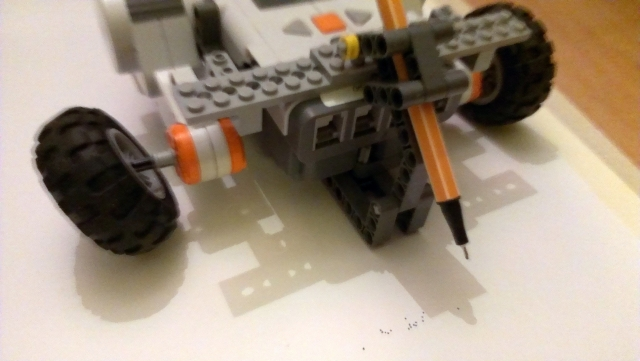
\includegraphics[width= 6cm]{img/wheel_failure.jpg}
 \caption{Image of the wheel failure}
 \label{fig:failure}
\end{figure}


\begin{itemize}
\item
\end{itemize}


\subsection{Data (see data.csv)}

\noindent
\csvautotabular[separator=semicolon]{data_ahead.csv}
\newline

\noindent
\csvautotabular[separator=semicolon]{data_left.csv}
\newline

\noindent
\csvautotabular[separator=semicolon]{data_right.csv}


%\begin{figure}
% \center
% \includegraphics[width= 6cm]{img/plot_left.jpg}
% \caption{Plot of the measurements of the left arc.}
% \label{fig:data_left}
%\end{figure}

%\begin{figure}
% \center
% \includegraphics[width= 6cm]{img/plot_right.jpg}
% \caption{Plot of the measurements of the right arc.}
% \label{fig:data_right}
%\end{figure}

%\begin{figure}
% \center
% \includegraphics[width= 6cm]{img/plot_ahead.jpg}
% \caption{Plot of the measurements of movement ahead.}
% \label{fig:data_ahead}
%\end{figure}

\section{Observations}
\subsection{Execution}


\subsection{Accuracy}
%including how you arrived at these estimates and why they are plausible.
\begin{itemize}
\item
\end{itemize}

\subsection{Precision}
%including how you arrived at these estimates and why they are plausible.
\begin{itemize}
\item
\end{itemize}

\section{Summary}
\subsection{}
\begin{itemize}
\item
\end{itemize}


%CONTENTS
%NOTES


%COPY AND PASTE FROM HERE

%\begin{enumerate}
% \item 
%\end{enumerate}

%\href{link}{text}

%\begin[Language=Python]{lstlisting}
%#PYTHON CODE HERE
%\end{lstlisting}

%\lstinputlisting[language=Java]{ }

%\csvautotabular[separator=semicolon]{data.csv}

%\begin{figure}
% \center
% \includegraphics[width= cm]{img/ }
% \caption{}
%\end{figure}

%BIBLIOGRPAHY?
\bibliographystyle{plain}%amsalpha
\bibliography{Top30.bib}
%\bibentry{}

\end{document}
